\documentclass{article}
\usepackage{graphicx}
\usepackage[margin=1.5cm]{geometry}
\usepackage{amsmath}

\begin{document}

\title{Warm Up: Objects in Free-Fall, Projectiles}
\author{Prof. Jordan C. Hanson}

\maketitle

\section{Memory}

\begin{enumerate}
\item $y(t) = -\frac{1}{2}g t^2 + v_{i,y} t + y_i$ ... Vertical displacement.
\item $v_y(t) = -g t + v_{i,y}$ ... Vertical velocity.
\end{enumerate}

\section{Objects in Free-Fall, Projectiles}

\begin{enumerate}
\item Note in Fig. \ref{fig:1} the initial velocity is broekn into the vertical and horizontal components.
\begin{figure}[ht]
\centering
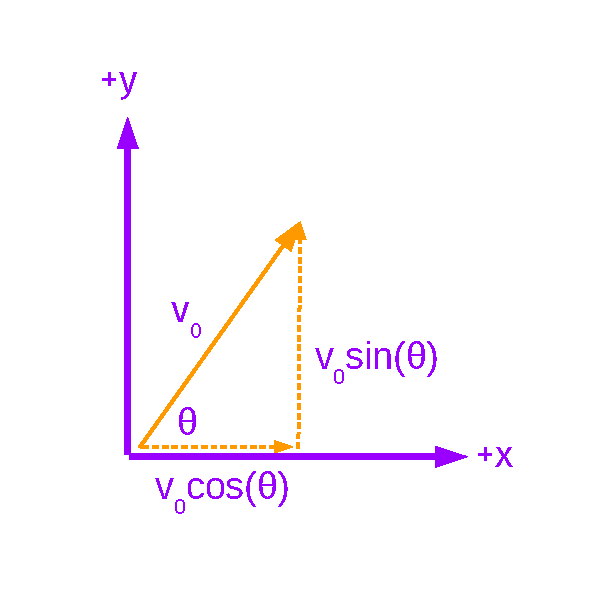
\includegraphics[width=0.33\textwidth,trim=0cm 1.25cm 0cm 1cm,clip=true]{figures/Vectors1.pdf}
\caption{\label{fig:1} The initial velocity $\vec{v}_0$ launched at an angle $\theta$ with respect to the x-axis.}
\end{figure}
\item Suppose an object is launched into the air from the origin at an angle $\theta$ with respect to the horizontal, with an initial velocity $\vec{v}_{i}$, eventually landing back at $y=0$.  Use the \textit{second} equation in the Memory bank to show that the total time spent in the air is 
\begin{equation}
T = \frac{v_i \sin\theta}{g} \label{eq:1}
\end{equation}
\item Use the \textit{first} equation in the Memory Bank to show that $T$ is given by Eq. \ref{eq:1}. \\ \vspace{5cm}
\item \textit{Hints: for the first exercise, ask yourself what the velocity is at the apex of the trajectory?  For the second exercise, solve the quadratic for the times that make $y=0$.}
\end{enumerate}

\end{document}
